\section{Experiment 2: Enhancing The Training Captions}
% Corresponging Progress Reports:
% https://www.notion.so/241220-Matthias-reducing-train-data-with-care-First-AI-captions-0a0a3c610dba4d9c84d4eda4fb1c53dd
% https://www.notion.so/250110-Matthias-AICaptions-Evaluation-053ef06c3e6e4858808c9266cc1bffc0
% https://www.notion.so/20250119-Matthias-Filling-The-gaps-2-a8f598e120de4b6ba4b20a7d0a2a9253#18e2cfd830264119bbfcd90d223b4cc0

\subsection{Background}

As shown in the previous chapter, the brain diffuser in particular has problems reconstructing the natural images and, even more so, generalising the learned translators to the artificial shapes test set. A pure diversity-based reduction (or possible extension) of the dataset does not seem to be sufficient to improve performance sufficiently. For this reason, the following section will focus on the reconstruction performance of the brain diffuser and how it can be improved. 

As described at the beginning, three different translators are trained with the brain-diffuser: for the VDVAE, the clipvision features and the cliptext features. The captions of the images that were used to gather the cliptext features were generated by using crowdsourcing (for the training data and for the natural test images) and partly manually created for this work (for the artificial shapes). It should be noted that the captions of the training images are all very short and usually focus on only a few prominent features of the images. It is possible that further details in the images may be completely ignored by the captions, or that descriptions of shapes, colours and lighting may not be considered at all. The generated test captions for the artificial shapes can be found in the provided github repo with together with the source-code for this study\cite{mildenbergerKamitaniLabBrain_diffuser}.

In the versatile diffusion process, which is used to generate the final images from the decoded brain activity, the decoded cliptext features are used to contextualise the diffusion process\cite{ozcelikNaturalSceneReconstruction2023,xuVersatileDiffusionText2024}. Due to the novelty of the versatile diffusion algorithm, little research has been done on how the cliptext context within this model affects the output images. However, diffusion-based image reconstruction algorithms that generate images from a prompt have been around for much longer\cite{rombachHighResolutionImageSynthesis2022,sahariaPhotorealisticTexttoimageDiffusion2022}, so we can at least refer to the research that examines the prompts used to control the diffusion-based models. In our model, the prompts used in the further diffusion process cannot be directly influenced, but the way in which the cliptext features that the translator reads from the brain activity are generated can be controlled by adapting the captions of the training data. It is therefore worth investigating how the diffusion process can be controlled with different prompts to better understand how our reconstruction can be improved. 

The process of searching for optimal prompts to optimise the output images of diffusion is called `prompt engineering'\cite{witteveenInvestigatingPromptEngineering2022}. This process itself is very difficult to operationalise because the quality assessment of the reconstructed images is sometimes a subjective process. Sometimes people are needed to provide a qualitative assessment of the results\cite{pavlichenkoBestPromptsTexttoImage2023}. The prompts can have a very strong influence on the generated images and steer the output in a certain direction by individual subtleties such as the repetition of single words,  the inclusion of individual high-level concepts within the prompt or a focus on low-level descriptive features (such as shapes, colours and structures)\cite{witteveenInvestigatingPromptEngineering2022}. One problem with diffusion-based image generation models is that they are not very good at generating images of concepts that are underrepresented in the training data set\cite{samuelGeneratingImagesRare2024}. The insight from the previous experiment and the research by Shirakawa et\ al.\cite{shirakawaSpuriousReconstructionBrain2024} has shown that in our case, too, the reconstruction of the artificial shapes in particular needs improvement. It can be assumed that such unnatural images tend to be underrepresented in the training datasets of the diffusion models\cite{schuhmannLAION400MOpenDataset2021, schuhmannLAION5BOpenLargescale2022}, and that a particular challenge is therefore to improve their reconstruction. To counteract this bias, this experiment investigates how the reconstruction of artificial shapes in particular can be improved by specifically modifying the labels of the training images. 

% - Auch wenn wir nicht direkt die prompts beeinflussen können, die am Ende rauskommen, sondern nur die cliptext embeddings, können wir indirekt steuern, wie diese aussehen mit den trainingsprompts
% - Überleitung vom Dropout Kapitel
    % - Insbesondere der brain-diffuser Algorithmus hatte Probleme und benötigt möglicherweise mehr als nur eine bessere Auswahl der Trainingsbilder
    % - Einerseits konnten wir die Ergebnisse für natural test images nicht verbessern, bei den Artificial Shapes sogar eher verschlechtern
    % - Wir wollen unsere Trainingsdaten also so enhancen, dass wir diese Probleme beheben können
% Was kann ich überhaupt hier für den Background schreiben?
% - Brain-diffuser besteht aus drei Teilen: VDAVE, cliptext und clipvision. In diesem Teil werden wir zunächst den cliptext Teil vornehmen
% - Die Captions wurden von Menschen generiert, die für Trainingsdaten und natural test Images von Crowdsourcing und die für die Artificial Shapes von mir selbst
% - Die Captions haben teilweise biase, sind teilweise falsch oder sehr kurz und beziehen sich in der Regel nur auf wenige Prominente Merkmale in dem Bild, könnten also noch verbessert werden
% - Aufgrund der recency gibt es noch nicht viel Forschung zu dem Einfluss auf die versatile diffusion, aber auf prompts in diffusion process an sich schon
    % - Der caption context in dem versatile diffusion model ist related zu den prompts die man eingeben kann
    % - Human in the loop Prozesse die dafür sorgen, dass die Prompts besser werden können, da es schwierig ist die Bildqualität automatisch zu bestimmen\cite{pavlichenkoBestPromptsTexttoImage2023}
    % - Unter anderem in vorigen Experimenten und bei Shirakawa et al. \cite{shirakawaSpuriousReconstructionBrain2024}, dass gerade Artificial Shapes mit zu viel naturalness gebiased werden da ein Fokus auf photorealistic images\cite{sahariaPhotorealisticTexttoimageDiffusion2022} \cite{rombachHighResolutionImageSynthesis2022} liegt.
    % - Man kann die Prompts unterscheiden in semantische und stylistic considerations. Nouns beeinflussen die image generation sehr stark. Man kann einzelne Wörter wiederholen und Fokus auf verschiedene Konzepte setzen \cite{witteveenInvestigatingPromptEngineering2022}. 
    % - In dem input Datensatz auf das die underlying diffusion trainiert wurde ist zu vermuten, dass natürliche Bilder den Großteil ausmachen \cite{schuhmannLAION400MOpenDataset2021} Auch noch schuhmann laion 5b aber findet der gerade irgendwie nicht.

% Related Works:
    % - Es ist schwierig, seltene Konzepte zu erstellen, die in den Trainingsdaten nicht so stark repräsentiert sind. \cite{samuelGeneratingImagesRare2024}. Die machen Seedselect, eine Methode mit der man versuchen kann den diffusion seed so zu setzen, dass rare concepts besser rekonstruiert werden können
    % -  Hier haben sie versucht mithilfe von KI einzelne Merkmale aus den Bildern rauszusuchen, welche den nachfolgenden Prozess besser guiden können \cite{Hu_2023_ICCV}

To my knowledge, there has been no detailed investigation of how a focus of captions of high-level concepts in an image versus low-level features of the images can differ in terms of how well either natural or unnatural images can be reconstructed. In particular, we found no study of how this focus on different image characteristics affects the reconstruction of out-of-subspace images (such as our artificial shapes) in relation to brain activity. The hypothesis of this experiment is that, on the one hand, the reconstruction performance of natural images can be improved if the captions of the training images focus on the high-level concepts of the images. On the other hand, the performance of the artificial images should be improved if the captions refer more to the low-level properties such as colour, shape and structure of the training data.


\subsection{Methods}
To further investigate the performance of the Brain Diffuser algorithm, the influence of the subtitles and the cliptext translator is first tested. Possible differences that may result from the high-level vs.\ low-level information of an image are to be analysed. For this reason, additional captions are created below for the training data, focusing on either the high-level or the low-level features of the image. The API of ChatGPT\cite{OpenAI_ChatGPT_2024} was used to generate the additional captions for the training images. With this, captions with two different prompts were generated for all 1200 training images. As it was empirically found that the cliptext features can encode less information with increasing number of tokens (= caption length)\cite{zhangLongCLIPUnlockingLongText2024}, care was taken to ensure that the length of the generated captions did not exceed 35 tokens as far as possible. The two prompts used to generate the subtitles are as follows
\begin{itemize}
    \item \textbf{high-level}: Describe the visual contents of this picture. Focus on the semantic concepts in the image. What are the main subjects of the image and what is happening in it? Make sure the output doesn't exceed 25 tokens.
    \item \textbf{low-level}: Describe the visual contents of this picture without using the word representing its direct category or semantic meaning as much as possible. Instead, focus on the colors, shapes, and textures with their relative positions in the image. Do not interpret the scene just describe what is actually visible. Make sure the output doesn't exceed 25 tokens.
\end{itemize}

The number of desired tokens per generated caption can only be specified implicitly via the prompt, without cutting off a caption in the middle. Accordingly, the number of tokens actually generated varies slightly. Captions longer than 35 tokens were excluded and the prompt was repeated until a corresponding caption shorter than 35 tokens was found. On average, 30.81 tokens (std = 2.8) were generated for the low-level captions and 22.84 (std = 3.17) for the high-level captions. The higher length of the low-level captions can be explained by the fact that semantic concepts, which can usually bundle many low-level properties (e.g.\ `dog' vs.\ `creature with four legs, fur and snout'), have to be avoided. Figure~\ref{fig:aicap_caption_samples} compares the high-level and low-level captions for two images from the training dataset with the human-generated captions. It can be seen that the low-level captions do indeed largely avoid semantic descriptions and tend to describe colours, shapes and textures. The high-level captions are comparatively similar to the human-generated captions and refer to semantic concepts (e.g.\ raccoon or can).

\begin{figure}[ht]
    \centering
    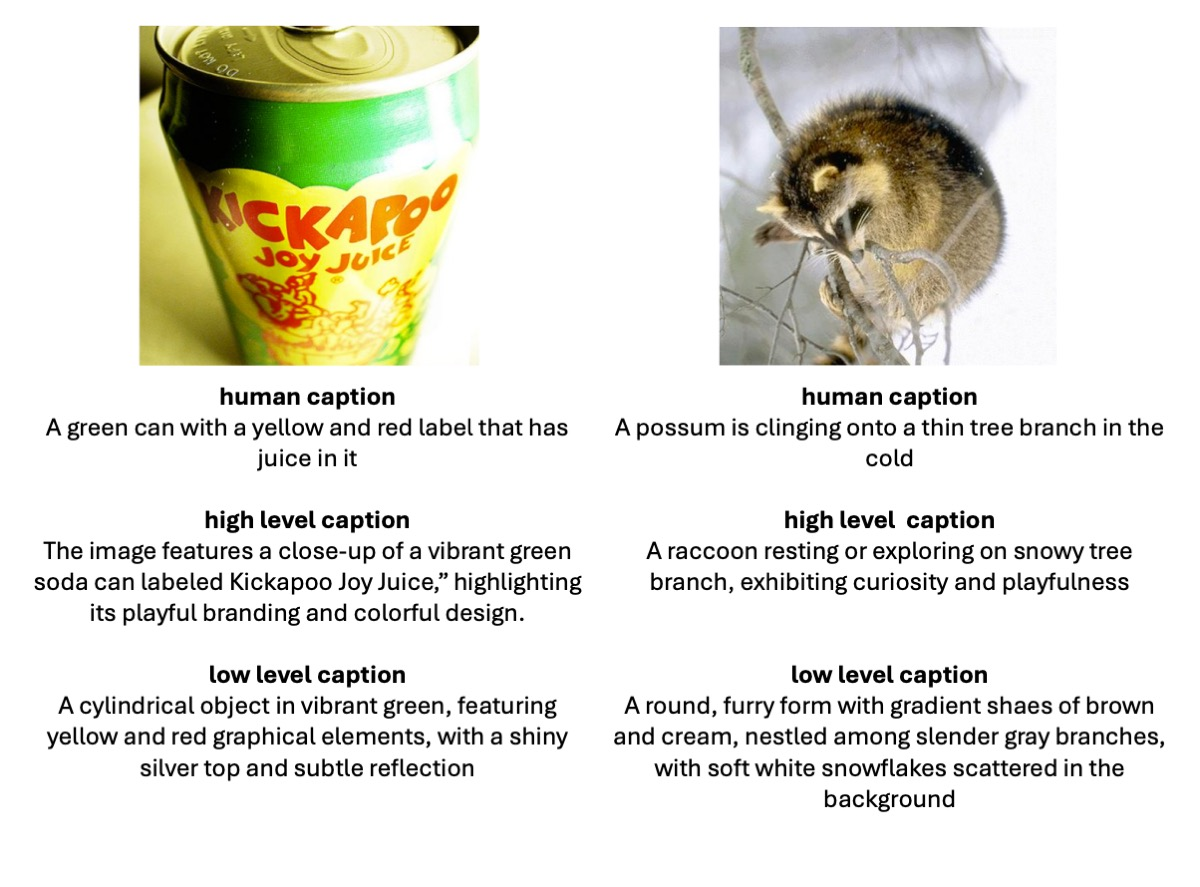
\includegraphics[width=1\textwidth]{plots/aicap_samples.jpeg}
    \caption{Captions with different prompts}\label{fig:aicap_caption_samples}
\end{figure}

The generated captions were subsequently used to train the Brain Diffuser's cliptext encoder. The clipvision and VDVAE components of the brain-diffuser do not change as a result, so only the performance of the cliptext translator is reported. For an extended baseline against which to compare the AI-generated subtitles, the human-generated subtitles are shuffled in an additional test condition. Thus, in this condition the captions have nothing to do with the actual image content, the translator should not be able to learn to make any meaningful predictions, just as the reconstructions produced with the translator trained with shuffled captions should be worse than with the normal baseline. In the Translator, the human-generated captions are used as test data for all comparisons to ensure comparability between conditions (i.e.\ the same test data is used for all conditions). 

When reconstructing with the Versatile Diffusion algorithm in the Brain Diffuser, the mixing parameter, which determines the influence of the cliptext features on the final reconstruction, is set to 0.4 and 0.8 respectively. In the original publication of the brain-diffuser\cite{ozcelikNaturalSceneReconstruction2023} the mixing parameter was 0.4, but in order to obtain a stronger influence of the captions and thus to be able to better evaluate the differences in the captions, the reconstructions are additionally analysed here with the parameter 0.8.


\subsection{Results}

\subsubsection{Translator Performance}

\begin{figure}[ht]
    \centering
    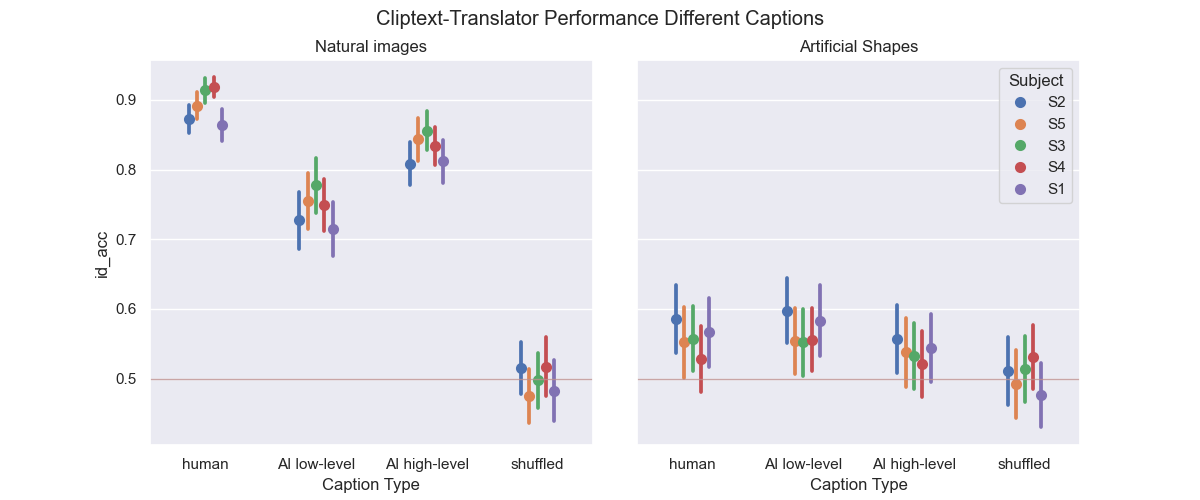
\includegraphics[width=0.9\textwidth]{plots/aicap_translator.png}
    \caption{Translator Performance for different Caption types}\label{fig:aicap_translator}
\end{figure}

Figure~\ref{fig:aicap_translator} shows the results of the cliptext translator for both the natural test images and the artificial shapes. The effects can be seen very clearly for the natural test images, the identification accuracy of the translator trained with the human-generated captions is the highest. This is not surprising, as the test data for all conditions were also the human-generated captions of the test images, and therefore there is a slight domain mismatch for the AI data captions (the training data is generated by the AI, the test data by humans). The translator trained with shuffled training data is exactly at random probability, so the cliptext features could rightfully not be predicted. Both conditions with the AI-generated test data are also significantly better than random probability, with the high-level captions performing slightly better than the low-level captions (as noted above, the high-level captions also have a higher agreement with the human-generated captions). 


The results for artificial shapes are very different. Again, shuffled training data can predict results only at the random level; all other translators also show improved performance compared to the shuffled test data (and thus improved performance compared to the random level). In this condition, however, the translators trained with AI-generated high-level captions perform worse than those trained with low-level captions. The translator trained on the human-generated captions also appears to outperform the AI-generated high-level captions, although the result is somewhat less clear. 

\subsubsection{Reconstruction Performance}


The quantitative performance of the reconstructions for the natural test images is shown in Figure~\ref{fig:aicap_reconstruction_test_both_mixings} and for the artificial shapes in Figure~\ref{fig:aicap_reconstruction_art_both_mixings}. The results for mixing parameters 0.4 and 0.8 are shown for each type of caption and metric. The natural test images show that the differences between the individual captions with a mixing parameter of 0.4 are very small. Even the reconstructions with shuffled captions are only slightly worse with a mixing of 0.4 than with valid captions. The differences only become apparent when comparing the results with a mixing of 0.8. First, it can be observed that the pixel correlation increases for all captions as the mixing parameter increases. This is the case even for shuffled captions. An increased influence of the cliptext features therefore increases the pixel correlation in any case, even if it is a semantically incorrect influence as in the case of the shuffled captions. In the case of Dreamsim and Clip Accuracy, on the other hand, performance decreases as the mixing  increases, especially in the case of shuffled captions. For human-generated captions and high-level captions, performance degrades less with increasing mixing (or even remains constant) than for low-level captions. 
\begin{figure}[ht]
    \centering
    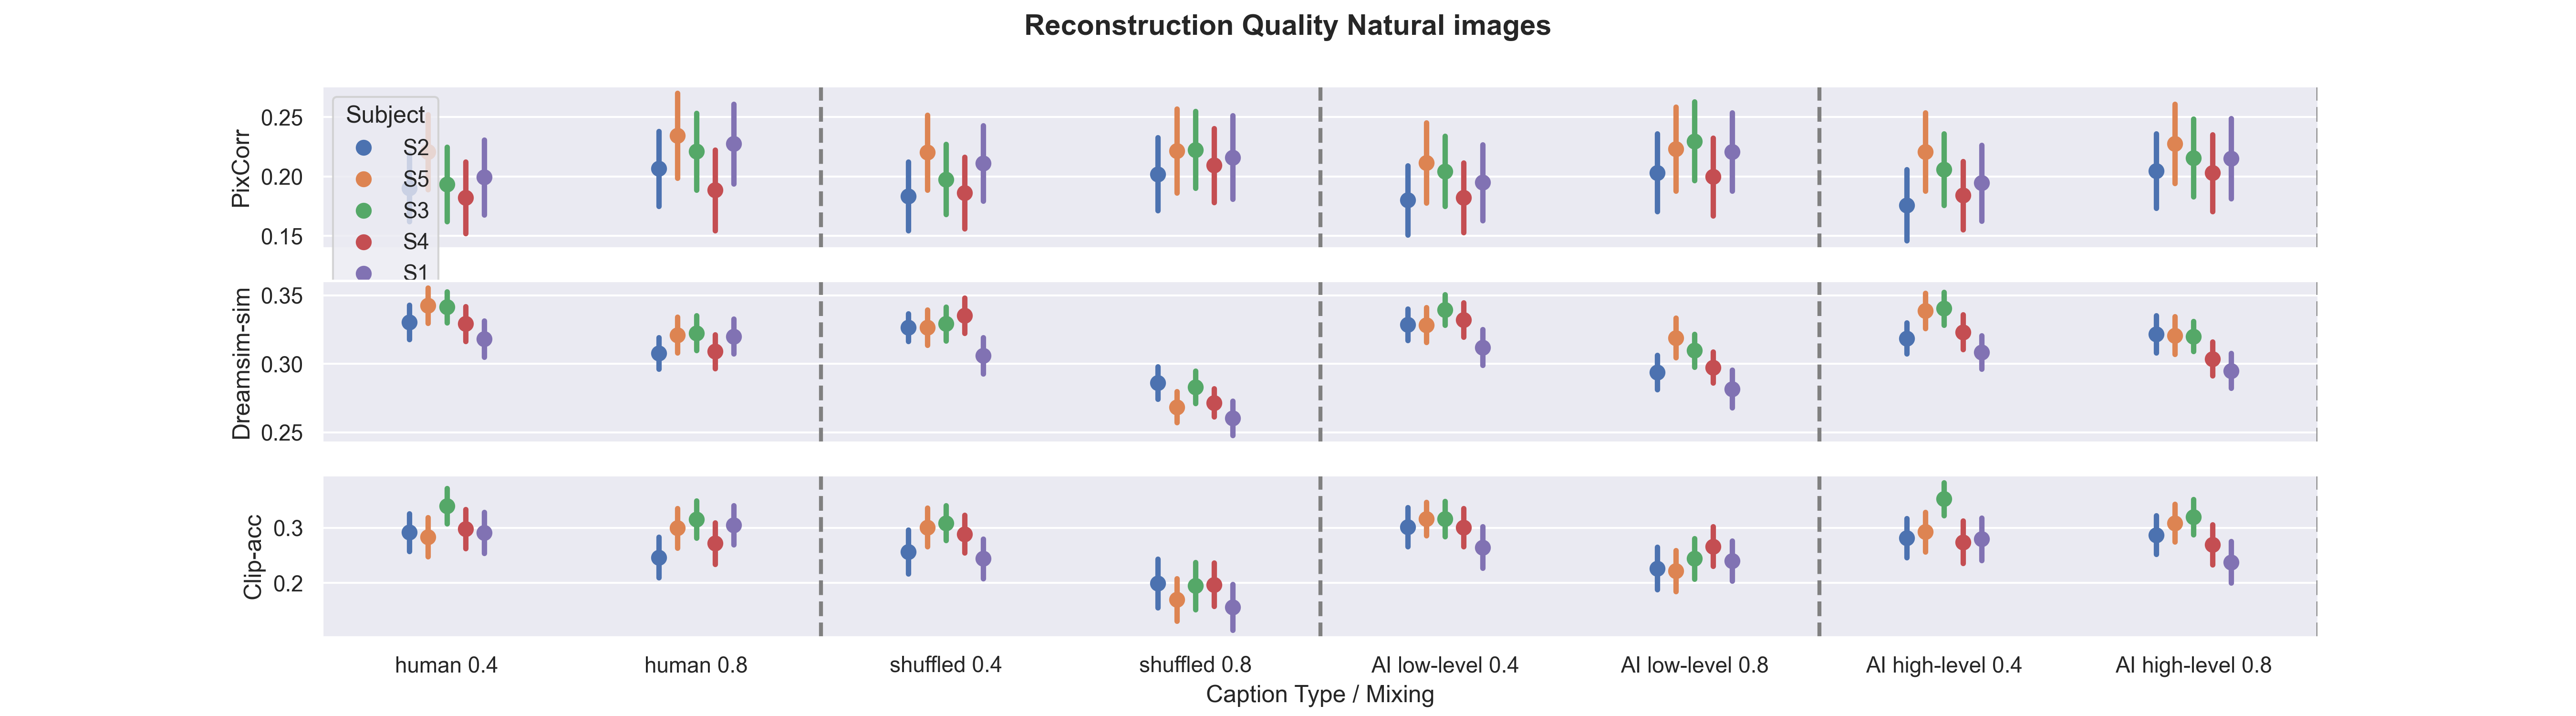
\includegraphics[width=1\textwidth]{plots/aicap_reconstruction_test_both_mixings.png}
    \caption{Reconstruction Natural Test Images with different captions}\label{fig:aicap_reconstruction_test_both_mixings}
\end{figure}


As before with the Translator, the results of the reconstruction of the artificial images are reversed. Again, with a low mixing of 0.4, there are very only few observable differences between the captions. And also as before, the pixel correlation increases with increasing mixing for all captions. But now, compared to the natural test images, the performance measured with Dreamsim Similarity also increases with increasing mixing for all captions. Especially with low level captions, good performance can be achieved with artificial images when mixing is high. The results for human and high-level captions are relatively similar and still significantly better than shuffled captions. The results for clip accuracy are very low and therefore difficult to interpret. As there is generally little semantic content in the artificial images, so the result is not surprising. 

\begin{figure}[ht]
    \centering
    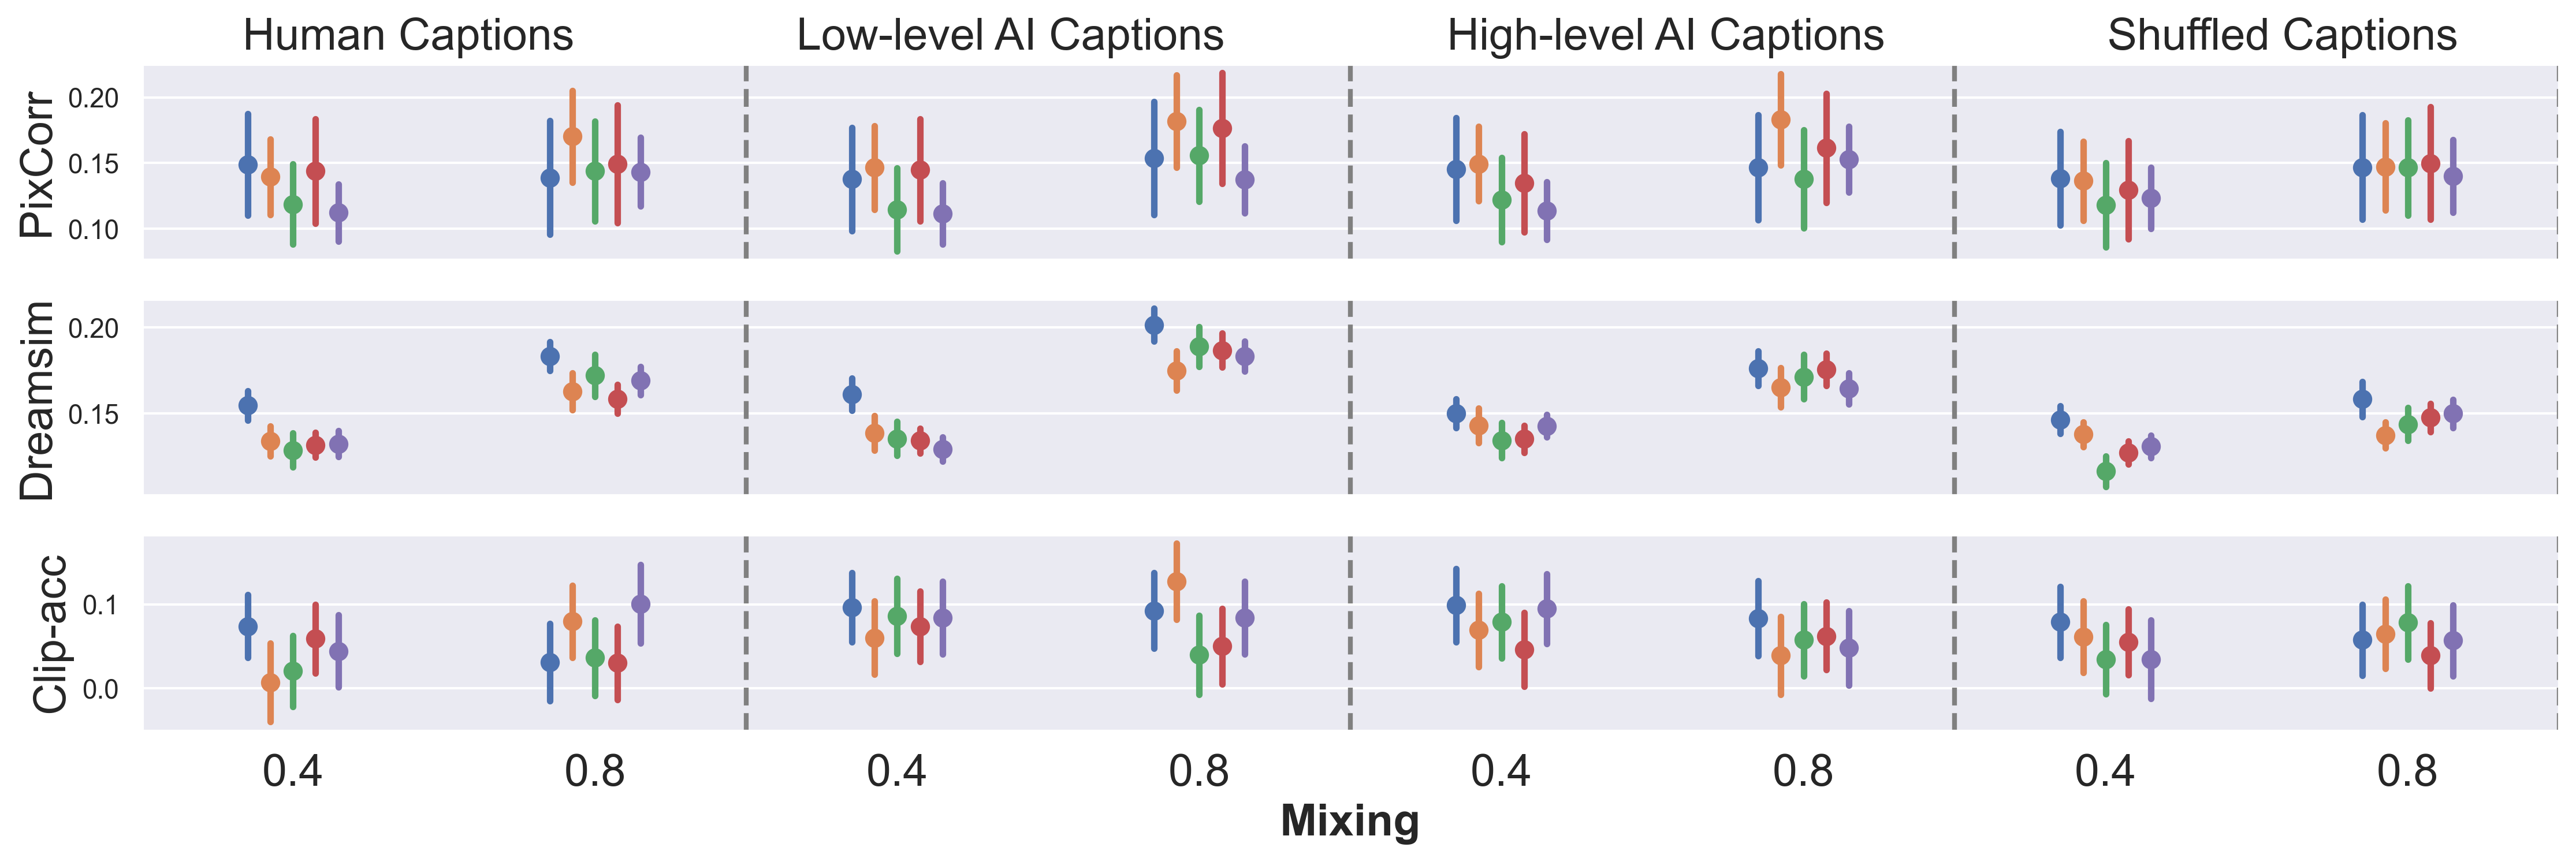
\includegraphics[width=1\textwidth]{plots/aicap_reconstruction_art_both_mixings.png}
    \caption{Reconstruction Artificial Images with different captions}\label{fig:aicap_reconstruction_art_both_mixings}
\end{figure}

\begin{figure}[ht]
    \centering
    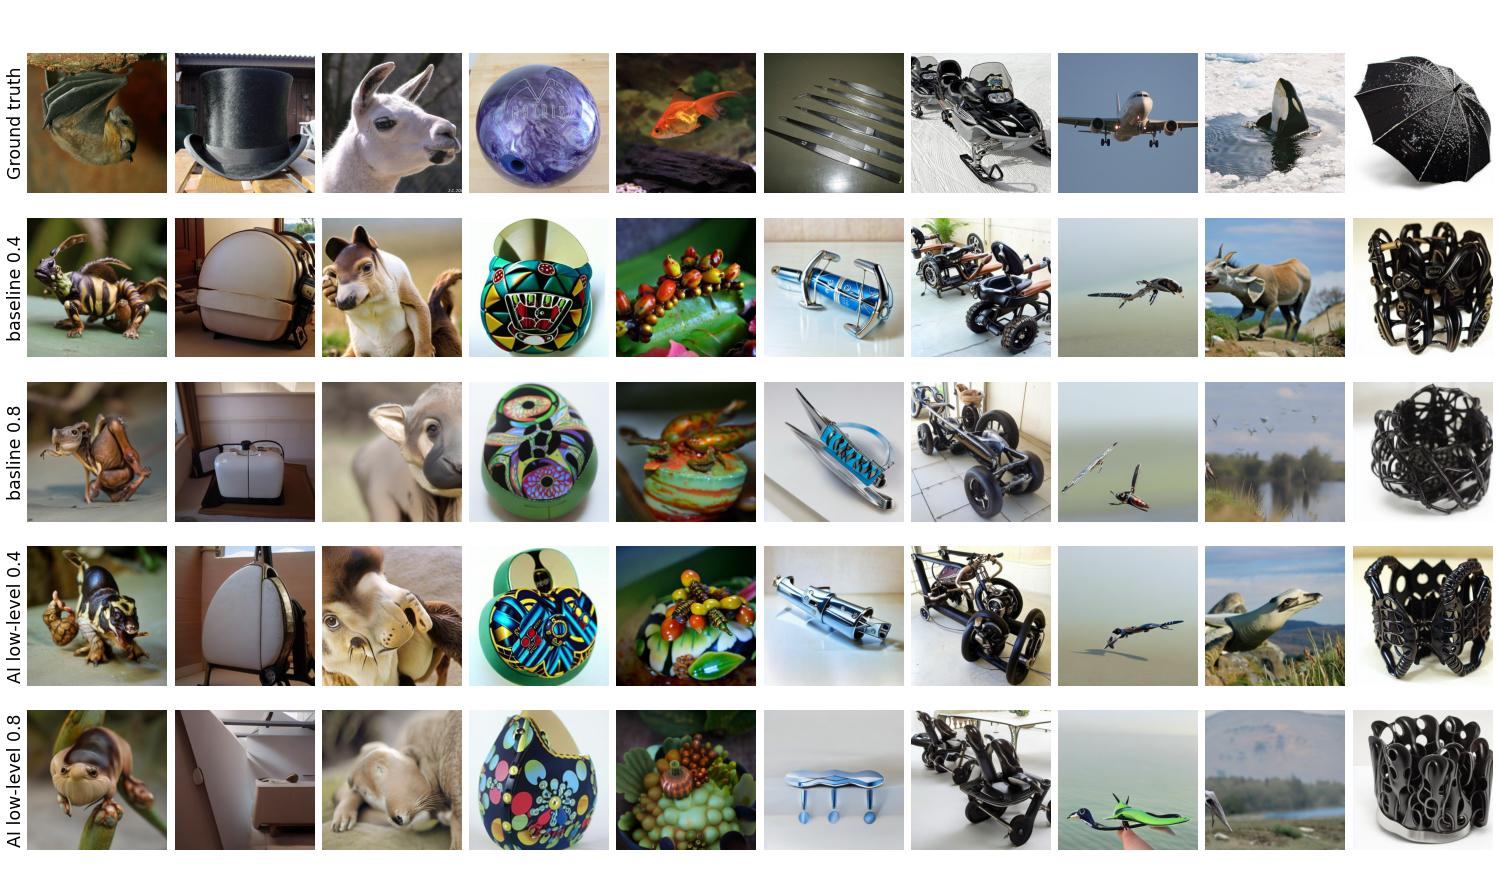
\includegraphics[width=1\textwidth]{plots/aicap_qual_test.JPEG}
    \caption{Qualitative Results for the low-level AI captions on Natural Test Images}\label{fig:aicap_qual_test}
\end{figure}

A qualitative comparison of the results with the low-level Ai generated captions with the baseline human captions for both mixing levels 0.4 and 0.8 can be seen in figure~\ref{fig:aicap_qual_test} for the natural test images and in figure~\ref{fig:aicap_qual_art} for the Artificial Shapes. The natural test images show that the images with higher mixing tend to be less detailed and less sharp (e.g.\ the llama or the killer whale). This suggests that higher levels of mixing are associated with poorer performance because the details of the objects are not as well represented. The differences between the 0.4 mixing baseline and the 0.4 mixing AI generated captions are more difficult to see. In the image with the snowmobile or the llama, it looks as if the low-level captions reduce the semantic meaning in the reconstructed images (the llama looks less like an animal, the snowmobile cannot be clearly identified as a vehicle). The effects that reduce performance for the natural test images have exactly the opposite effect for the artificial shapes in Figure~\ref{fig:aicap_qual_art}. Again, we see that the images with higher mixing are less detailed (e.g.\ in the purple cross where distinct people could be identified at low mixing and only shapes with high mixing). As with the natural test images, it can be observed that it is more difficult to find semantic meanings for the generated images in the reconstructions with the low-level AI captions (for example, in the case of the blue-grey cross, a hand can still be seen in the baseline and a landscape in the background; in the case of the reconstructions with the AI captions, it is more difficult to find semantic concepts for the reconstruction). In summary, the combination of reduced detail with higher mixing and the reduced semantic content of the images with the low-level AI captions results in better reconstruction of the artificial shapes in contrast to the baseline.Since the high-level captions from the AI yielded very similar results than the baseline captions (because the captions itself were very similar), there are not visible differences in the reconstructed images. A qualitative comparison can be found in the Appendix in figure~\ref{fig:aicap_qual_art_highlevel_appendix} for the natural test images and in figure~\ref{fig:aicap_qual_test_highlevel_appendix} for the artificial shapes.


\begin{figure}[ht]
    \centering
    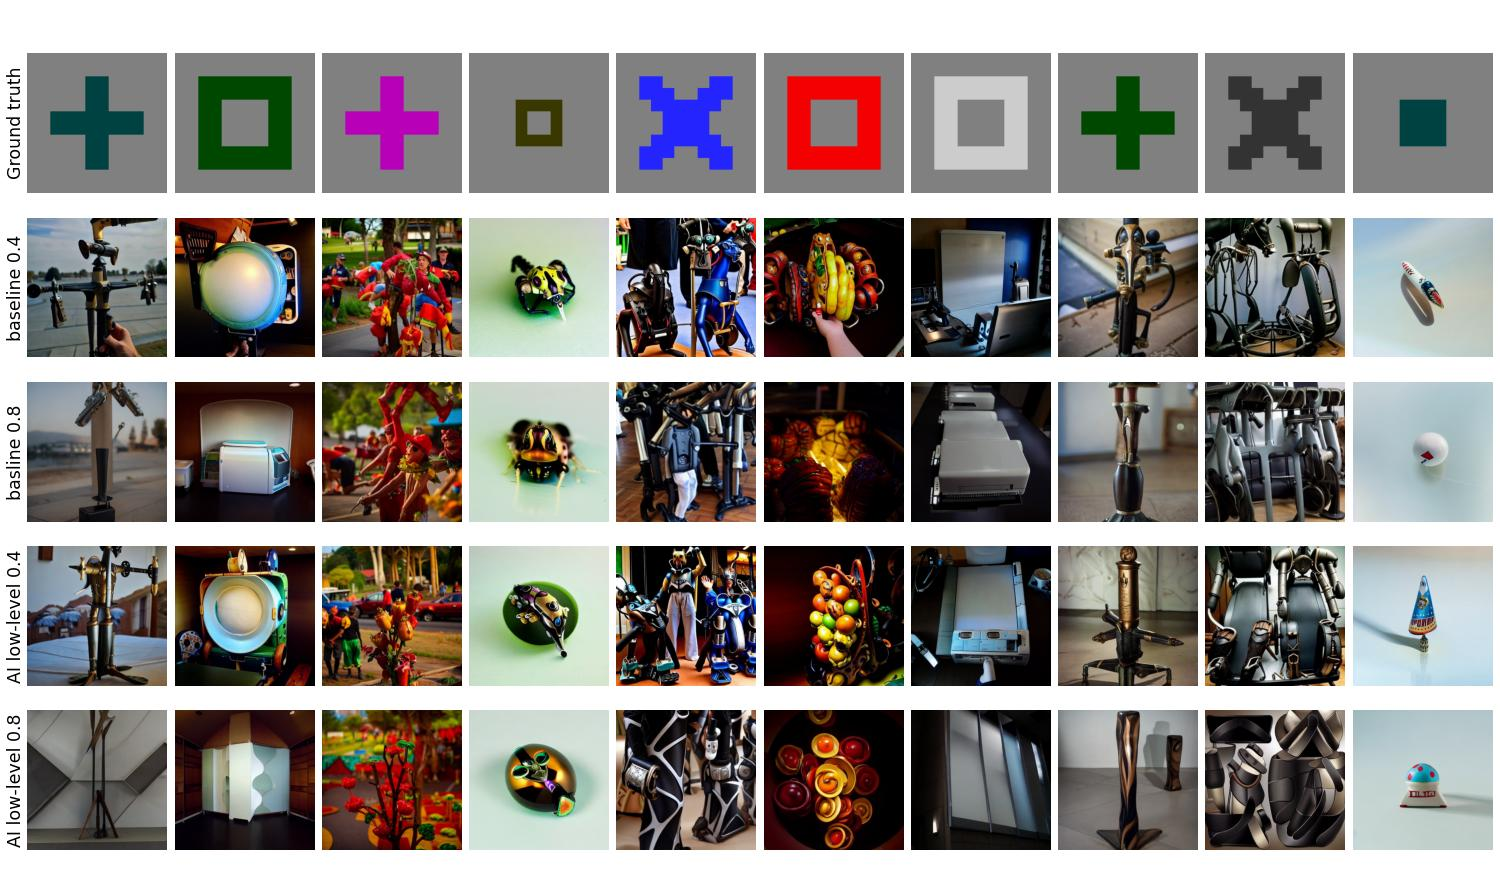
\includegraphics[width=1\textwidth]{plots/aicap_qual_art.JPEG}
    \caption{Qualitative Results for the low-level AI captions on Artificial Shapes}\label{fig:aicap_qual_art}
\end{figure}

\subsection{Discussion}

It could be shown that different types of captions, which refer to different features of the image, have a heterogeneous influence on the reconstruction performance. On the one hand, the hypothesis was confirmed, that captions in the training data that refer to low-level features of the images can also ensure that the artificial shapes (which themselves do not carry much high-level information) can be better reconstructed. On the other hand, the reconstruction performance for natural images (which carry a lot of semantic meaning) was not reduced,  when the labels referred to the high-level information of the training images, however it was also not improved. A reason for this could be a ceiling effect for the cliptext translator (as the results determined by the identification-accuracy are very high already in the baseline) or the fact, that the human generated captions are very similar to the AI generated high-level captions in the first place. PixelCorrelation did not prove to be a particularly good metric in this experiment, as it was able to detect an improvement in performance with increasing mixing in all cases (even with shuffled captions). The Dreamsim metric, on the other hand,  demonstrated the effect described above the strongest (low-level captions are good for artificial shapes and bad for natural test images). 

\begin{figure}[ht]
    \centering
    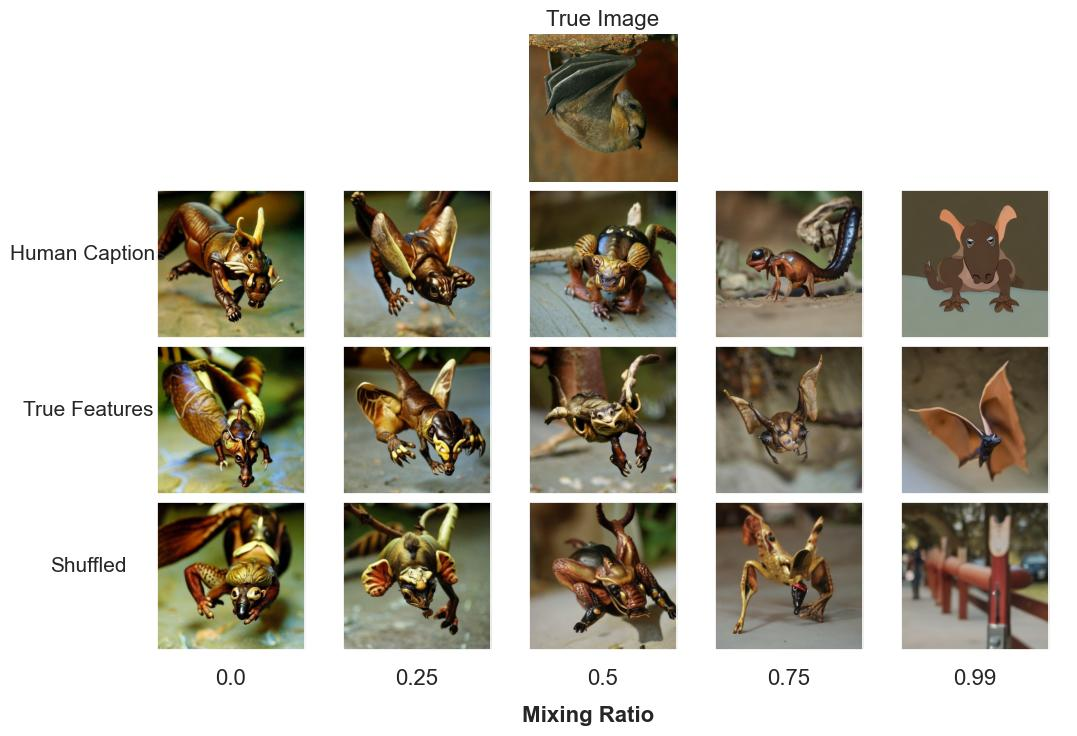
\includegraphics[width=0.8\textwidth]{plots/aicap_reconstruction_evolution_test_0.JPEG}
    \caption{Qualitative influence of different mixing ratios}\label{fig:aicap_reconstruction_evolution_test_0}
\end{figure}

For the natural test images and the artificial images, contrary effects were found as to whether increased mixing degrades (natural images) or improves (artificial shapes) the reconstruction performance. In order to identify the reason for this, a further analysis focused on the mixing parameter was conducted. Figure~\ref{fig:aicap_reconstruction_evolution_test_0} (and in the appendix in Figure~\ref{fig:aicap_reconstruction_evolution_art_0}) shows reconstructed images with increasing mixing ratios. In addition to the human and shuffled captions, the true features (i.e.\ the extracted clip text features of the images) are also used. It can be seen that as the mixing ratio increases, there is less detail in the image and the result becomes more blurred. This could be an explanation for the fact that the reconstruction performance (measured with dreamsim) for the natural test images decreases as the mixing ratio increases: because there is less detail in the reconstructed images, they are less reminiscent of photorealistic images (the effect of the decreasing performance is shown quantitatively in Figure~\ref{fig:aicap_reconstruction_quant_evolution_test} in the appendix). This could also be the reason why the performance for the artificial images generally increases as the mixing ratio increases: because there is less (hallucinated) detail in the reconstructed images, the similarity to the low-detail artificial images increases (the increasing performance for the artificial images is shown in a quantitative manner Figure~\ref{fig:aicap_reconstruction_quant_evolution_art} in the appendix). Also it's worthhile to note, that the semantic value of the images could not be increased for the high-level captions with increased mixing, even though these captions should have a focus on the semantic content of an image. Thus one an conclude, that using the cliptext features to increase the semantic value of the images will not be enough by itself.

To further investigate the influence of captions on reconstruction performance in the brain diffuser, further insights could be drawn from research on prompt engineering. The prompts used in this work (high-level and low-level) to instruct chatgpt how to create the image captions were purely subjectively formulated. Instead, an optimisation such as that used by Wen et al.\cite{wenHardPromptsMade2023} could be used to further tune the captioning to better highlight certain features in the input images. It would also not be necessary to use chatGPT as the method for creating the captions, other image captioning methods could be used instead. For example, a clipvision encoder could be used to generate initial embeddings of the training data, which could then be adapted using prompt engineering tools to highlight certain features of the image. These in turn could be converted into human readable text (`hard prompts')\cite{wenHardPromptsMade2023}. Methods such as PromptCap\cite{Hu_2023_ICCV} could be used to control the caption generation process to focus on particular features in an image, so that either semantic concepts or low-level features could be given more weight. This approach could also be used to systematically investigate which types of features are better or worse predicted by brain activity. 

In addition, it would be possible within the versatile diffusion algorithm\cite{xuVersatileDiffusionText2024} to provide multiple contextualisation with different caption types, so that both high-level and low-level features could be taken into account. However, it would be particularly important to investigate whether the addition of one would not in turn affect the other part of the reconstruction. In summary, the results of this experiment show that the reconstruction of images can be significantly influenced by changing the captions, but that this is particularly possible by strongly mixing the cliptext features in the versatile diffusion process. The side effect of this is that the naturalness of the images is generally reduced. 

% Outlook:
% - die Prompts direkt mit chatgpt zu generieren muss nicht die einzige sein, wie man den approach nutzen kann
    % - Es könnte noch mehr prompt-engineering betrieben werden um herauszufinden wie die rekonstruierten Bilder optimiert werden könnten
    % - Either hard prompt or soft prompts (es müssen ja gar keine captions generiert werden, es reichen die cliptext features)
% - Neue Methode um hard Prompts zu designen \cite{wenHardPromptsMade2023}
    % - Unterschied zwischen hard prompts und soft prompts
    % - Prompt Optimierung nach ChatGPT
    % - Es könnten die Prompts noch weiter darauf optimiert werden, sich auf bestimmte Merkmale in den Bildern zu fokussieren
    % - Sowas wie prompt cap könnte genutzt werden um noch besser darauf achten zu können, wie die prompts erstellt werden sollen \cite{Hu_2023_ICCV}
        % - Intermediate prompt optimization technique to guide the chatgpt output

% - Könnten auch die prompts komplett droppen und einen anderen diffusion approach benutzen\cite{xuPromptFreeDiffusionTaking2024,xuVersatileDiffusionText2024}
%     - Wir brauchen gar keinen Text unbedingt. Auch bei versatile diffusion nicht, dort geht es ja insbesonere um die cliptext features. 
%     - Context nur durch Bilder geben (weil der semantische Inhalt durch die cliptext features eh nicht besonders stark erhöht werden kann)
%     - Man könnte also auch doppelten Context geben durch Bilder
%     - Oder doppelten Text context
%     - Theoretisch sind viele Contexts möglich bei dem versatile diffusion approach, mit einer weiterentwicklung könnte man so dann auch je nach image das regeneriert werden soll ganz unterschiedlichen kontext geben


